\documentclass[11pt, a4paper]{article}

\usepackage[T2A]{fontenc}		%cyrillic output
\usepackage[utf8]{inputenc}		%cyrillic output
\usepackage[english, russian]{babel}	%word wrap
\usepackage{amssymb, amsfonts, amsmath}	%math symbols
\usepackage{mathtext}			%text in formulas
\usepackage{geometry}			%paper format attributes
\usepackage{fancyhdr}			%header
\usepackage{graphicx}			%input pictures
\usepackage{tikz}				%draw pictures
\usetikzlibrary{patterns}		%draw pictures: fill
\usepackage{enumitem}			%enumarate parameters

\geometry{left=1cm, right=1cm, top=2cm, bottom=1cm, headheight=15pt}
\setlist[enumerate]{leftmargin=*}	%remove enumarate indenttion
\sloppy							%correct overfull

\newcommand{\head}[4]
{
	\pagestyle{fancy}
	\fancyhf{}
	\chead{#3, #4}

	\begin{center}
	\begin{large}
	#1 \\
	\textit{#2}\\
	\end{large}
	\end{center}

}

\begin{document}

\head{Открытая студенческая олимпиада по математике \\ Казахстанского филиала МГУ}{19 декабря 2015}{Казахстанский филиал МГУ имени М. В. Ломоносова}{г. Астана}

\begin{enumerate}

\item (Абдикалыков А.К.) Пусть $z_n=a_nb_n-x_ny_n$. Видно, что $z_n$ можно представить в виде $z_n=\alpha n^2+\beta n+\gamma$ для некоторых постоянных $\alpha$, $\beta$, $\gamma$. Но так как $z_n$ обращается в ноль при трёх различных $n$, то $\alpha=\beta=\gamma=0$, и $z_n$ тождественно равно нулю.

\item Ответ: 12090. Положим $n$ простым: $f(n) = f(1) - f(n)$. То есть 
$$f(p) = \frac{1}{2}f(1)$$
для любого простого $p$.

Положим $n = p_1^{\alpha_1} p_2^{\alpha_2} ... p_s^{\alpha_s}$ и обозначим 
$$k(n) = \alpha_1 + \alpha_2 + ... + \alpha_s.$$
Несложно показать, что:
$$f(n) = \left( 1 - \frac{k(n)}{2} \right) f(1).$$
Имеем $2015 = 5^1 \cdot 13^1 \cdot 31^1$ и $2016 = 2^5 \cdot 3^2 \cdot 7^1$. Соответственно $k(2015) = 3$, $k(2016) = 8$.

\item Ответ: $f(x) \equiv 0$. Пусть $n \in \mathbb{Z}$. Тогда $f'(n) = f'(n+1) = 0$, откуда $f(n) = f(n+1) = 0$. Докажем от противного, что $f(x) = 0$ для всех $x \in [n, n+ 1]$. Пусть $x_0 \in (n, \,n+1)$ и $f(x_0) \neq 0$, например, $f(x_0) > 0$. Т.к. $f$ дифференцируема, то $f$ --- непрерывна на $[n, n+1]$. По теореме Вейерштрасса у нее существует максимум на $[n, n+1]$: 
$$f(x_1) = \max\limits_{[n, n+1]} f(x) > 0 \text{ и } x_1 \in (n, n+1).$$

По теореме Ферма имеем: $f'(x_1) = 0$, откуда $f(x_1) = 0$ --- противоречие.

\item Так как парабола является коническим сечением, то можно осуществить проективное преобразование с точкой в вершине соответствующего конуса, переводящее параболу в окружность. Дан вписанный четырехугольник $B_1B_2B_3B_4$. Касательные в $B_1$ и $B_2$ пересекаются в точке $K$, касательные в $B_3$ и $B_4$ в точке $L$. Осталось доказать, что $KL$, $B_1B_3$ и $B_2B_4$ пересекаются в одной точке.

\begin{center}
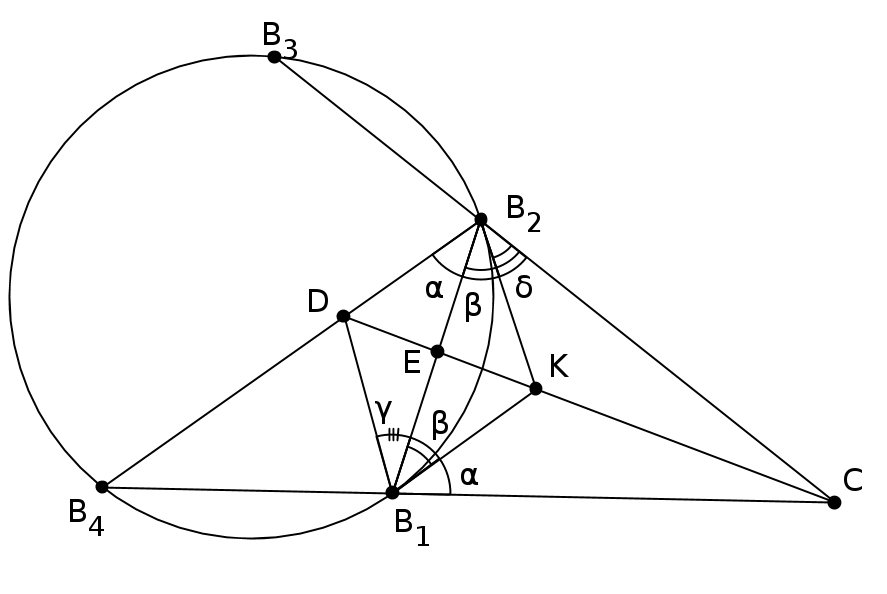
\includegraphics[width=0.8\linewidth]{pictures/2015-2016-4}
\end{center}

Пусть $C$ --- точка пересечения $B_1B_4$ и $B_2B_3$. $E$ и $K$ --- точки пересечения $CK$ с $B_1B_2$ и $B_4B_2$. Обозначим $\angle DB_2E = \angle CB_1K = \alpha$, $\angle EB_2K = \angle EB_1K = \beta$, $\angle KB_2C = \delta$ и $\angle DB_1B_2 = \gamma$. Выпишем двойные отношения (по теоремам синусов) от вершин $B_1$ и $B_2$ соответственно:
$$ \frac{\sin{\alpha}}{\sin{\beta}}: \frac{\sin(\alpha+\beta+\gamma)}{\sin{\gamma}} = \frac{CK}{KE} : \frac{CD}{DE}$$

$$\frac{\sin{\delta}}{\sin{\beta}}: \frac{\sin(\alpha+\beta+\delta)}{\sin{\alpha}} = 
\frac{CK}{KE} : \frac{CD}{DE}$$

Откуда получаем $\delta = \gamma$, то есть $D$ --- точка пересечения диагоналей. Аналогично доказывается, что $D$ лежит на $CL$. Итог: $KL$ проходит через точку пересечения диагоналей.

\item (Абдикалыков А.К.) Ответ: $-3\pi$. 

Очевидно, что $x=-3\pi$ является одним из решений. Введём функцию $f(x)=2x+\sin x$. Тогда данное уравнение можно переписать в виде $f(f(x))=-12\pi$. Поскольку функция $f(x)$ (а значит, и функция $f(f(x))$ вместе с ней) является возрастающей, то это уравнение не может иметь больше одного корня.

\item Каждому числу $a_j$ сопоставим ребро, соединяющее вершины графа с номерами $j$ и $a_j$. Полученный мультиграф имеет $n$ вершин и $n$ рёбер, и, следовательно, обязан содержать цикл. Номера вершин, входящих в любой из циклов, формируют требуемое подмножество $P$.

\item (Абдикалыков А.К.) Ответ: $(1)$ --- матрица порядка 1. Если порядок матрицы $n>1$, то из $\mathrm{rg}\,A=1$ следует вырожденность матрицы $A$, что, в свою очередь влечёт присутствие собственного значения 0. Так как след равен сумме всех собственных значений, то $\mathrm{tr}\,A=0$ --- противоречие. Удовлетворять всем условиям задачи может только матрица первого порядка, единственный элемент которой равен 1.

\end{enumerate}

\end{document} 
